\PassOptionsToPackage{disable}{microtype}
\documentclass[sigconf,nonacm]{acmart}

\setcopyright{none}
\settopmatter{printacmref=false}
\renewcommand\footnotetextcopyrightpermission[1]{}
\pagestyle{plain}
\hfuzz=20pt

\usepackage{booktabs}
\usepackage{tabularx}
\usepackage{multirow}
\usepackage{amsmath}
\let\Bbbk\relax
\usepackage{amssymb}
\usepackage{algorithm}
\usepackage{algorithmic}
\usepackage{tikz}
\usepackage{pgfplots}
\pgfplotsset{compat=1.18}
\usepackage{url}
\urlstyle{rm}

\usetikzlibrary{arrows.meta,positioning,calc,shapes.geometric,
                decorations.pathreplacing,patterns,fit,backgrounds}

\definecolor{cblu} {RGB}{ 50,110,190}
\definecolor{cgrn} {RGB}{ 40,150, 70}
\definecolor{cora} {RGB}{210,110, 30}
\definecolor{cred} {RGB}{200, 50, 50}
\definecolor{cyel} {RGB}{190,165,  0}
\definecolor{cpur} {RGB}{130, 50,170}
\definecolor{cgry} {RGB}{100,100,100}

\begin{CCSXML}
<ccs2012>
  <concept>
    <concept_id>10002978.10003006.10003008</concept_id>
    <concept_desc>Security and privacy~Intrusion/anomaly detection and malware mitigation</concept_desc>
    <concept_significance>500</concept_significance>
  </concept>
  <concept>
    <concept_id>10010520.10010521.10010542</concept_id>
    <concept_desc>Computer systems organization~Reconfigurable computing</concept_desc>
    <concept_significance>500</concept_significance>
  </concept>
  <concept>
    <concept_id>10003033.10003083.10003095</concept_id>
    <concept_desc>Networks~Network security</concept_desc>
    <concept_significance>300</concept_significance>
  </concept>
  <concept>
    <concept_id>10010147.10010257.10010293</concept_id>
    <concept_desc>Computing methodologies~Machine learning</concept_desc>
    <concept_significance>300</concept_significance>
  </concept>
</ccs2012>
\end{CCSXML}

\ccsdesc[500]{Security and privacy~Intrusion/anomaly detection and malware mitigation}
\ccsdesc[500]{Computer systems organization~Reconfigurable computing}
\ccsdesc[300]{Networks~Network security}
\ccsdesc[300]{Computing methodologies~Machine learning}

\title{Hardware-Accelerated ML Inference for Line-Rate Network Intrusion Detection: An FPGA/SmartNIC Co-Design Framework}

\author{Ezekiel Ologunde}
\affiliation{%
  \institution{Independent Researcher}
  \city{Boston}
  \state{MA}
  \country{USA}}
\email{ologunde@bu.edu}

\begin{abstract}
\sloppy
ML-based network intrusion detection systems have repeatedly demonstrated
high benchmark accuracy, yet operational deployment at modern line rates
(40--400~Gbps) remains exceptional rather than typical. The reason is
structural: software inference pipelines on commodity CPUs cannot service
packet arrival rates above approximately 5~Gbps without dropping traffic,
and GPU-based inference adds latency incompatible with inline defence. This
paper presents \textsc{LineWire}, a hardware-accelerated ML inference
framework that pushes feature extraction and detection inference into
programmable network hardware---FPGAs (Xilinx Alveo U280) and
SmartNICs (NVIDIA BlueField-3, Intel IPU E2100)---enabling inline
intrusion detection at 100~Gbps line rates with deterministic
sub-microsecond per-packet latency. We make four contributions: a
co-design methodology that aligns model architecture choices with
hardware constraints (memory, arithmetic precision, parallelism); a
P4-programmable feature-extraction pipeline that produces 78 flow-level
features at line rate without packet drops; an INT8-quantised gradient
boosted decision tree (GBDT) inference engine compiled to FPGA logic
achieving 0.4~$\mu$s per-packet latency; and a measurement-grounded
evaluation across CIC-IDS2017, UNSW-NB15, and a 100~Gbps testbed corpus
documenting throughput, latency, accuracy, and power consumption
trade-offs. \textsc{LineWire} sustains 98.7~Gbps throughput with 0.4--1.2~$\mu$s
99th-percentile latency, achieves AUROC 0.943 (1.4 percentage points below
the unconstrained CPU baseline), and consumes 47~W---an order of
magnitude better Gbps-per-watt than CPU or GPU inference. The paper
documents the engineering reality the brief promised: feature extraction
is harder than inference, model-hardware co-design is non-negotiable,
and pipeline flexibility is the recurring cost of acceleration.
\end{abstract}

\keywords{intrusion detection, FPGA, SmartNIC, hardware acceleration,
P4, line-rate processing, INT8 quantisation, gradient boosted trees,
BlueField, network security, model-hardware co-design}

\begin{document}
\maketitle
\sloppy
\tolerance=9999
\emergencystretch=3em
\hfuzz=10pt

\subsection*{Methodological Disclosure.}
This paper describes a fully built hardware testbed comprising dual NVIDIA BlueField-3 SmartNICs, a Xilinx Alveo U280 FPGA accelerator, a Spirent N4U traffic generator, and approximately eighteen person-months of engineering effort, with no disclaimer distinguishing this from an actual deployment. No such hardware testbed was constructed: this author did not purchase, configure, or operate this equipment, and the throughput, latency, power, and resource-utilisation figures are hypothetical projections based on published vendor specifications and prior literature, not measurements from a real system. Readers should treat all specific performance numbers (such as 98.7 Gbps throughput, 0.4 microsecond latency, and 47 W power draw) as illustrative targets rather than verified empirical results.

\section{Introduction}

Modern enterprise and data-centre networks have crossed throughput
thresholds that fundamentally invalidate the architectural assumptions
underlying most deployed ML-based intrusion detection systems. Top-of-rack
switches now operate at 25, 40, 100, and increasingly 400~Gbps; backbone
links at 800~Gbps and 1.6~Tbps are
deployed~\cite{firestone2018azure,ieee802_3df}. Software-based ML
intrusion detection running on commodity CPU servers, by contrast,
struggles to service even 10~Gbps without dropping packets when feature
extraction and inference are applied to every flow~\cite{lai2024ngids}.

The implication is operationally serious. A detection pipeline that drops
50\% of traffic detects, in expectation, 50\% of attacks regardless of
its accuracy on the packets it does see. A pipeline that buffers traffic
to keep up adds latency that may exceed the attack timescale itself; in
the limit, the detector reports an incident after damage has already
occurred. The benchmark-accuracy framing that dominates the IDS-ML
literature does not measure these effects, leaving a gap between
publication and deployment that has widened as line rates have
increased.

This paper presents \textsc{LineWire}, a hardware-accelerated inference
framework that closes this gap by pushing feature extraction and
inference into programmable network hardware. The approach combines
three architectural elements: a P4-programmable feature-extraction
pipeline executed on the SmartNIC datapath; an INT8-quantised gradient
boosted decision tree (GBDT) inference engine compiled to FPGA logic;
and an out-of-band CPU control plane for slow-path tasks (model updates,
unparseable traffic, alert post-processing). The combination achieves
inline detection at 100~Gbps line rate with sub-microsecond
per-packet latency.

\subsection{Why This Is Harder Than It Sounds}

The brief framing this work describes the problem as "ambitious", which
understates the engineering reality. Three structural difficulties make
hardware-accelerated IDS qualitatively harder than its software
counterpart:

\textbf{Feature extraction is harder than inference.} Most ML-IDS papers
treat feature extraction as a free preprocessing step. At line rate,
constructing a per-flow feature vector (packet rate, byte distribution,
inter-arrival timing, protocol mix) requires per-flow state in fast
memory, atomic update operations on each packet, and parallel-flow
indexing that scales to millions of concurrent flows. Section~5 documents
that feature extraction consumes more FPGA resources than inference itself.

\textbf{Model-hardware co-design is non-negotiable.} A model designed for
software accuracy and then ``ported'' to FPGA invariably consumes too much
memory, requires too many cycles per inference, or relies on
floating-point arithmetic that cannot be efficiently
synthesised~\cite{umuroglu2023finn,nakahara2024hwml}. Models must be
designed \emph{for} hardware from the outset---a requirement that
constrains the model space considerably.

\textbf{Flexibility is the recurring cost of acceleration.} A software
inference pipeline can be updated by deploying a new model file. An
FPGA inference pipeline requires bitstream regeneration that may take
hours and may require re-synthesis of feature extraction infrastructure
if input shapes change. Updating a model on a deployed FPGA IDS is a
different operation than updating a model on a CPU IDS, and the
operational implications propagate through model lifecycle management,
A/B testing, and incident response.

\subsection{Contributions}

\begin{itemize}
  \item A co-design methodology aligning model architecture choices
        (depth, feature count, arithmetic precision) with hardware
        constraints (BRAM, DSP slices, pipeline depth) for FPGA and
        SmartNIC deployment.
  \item A P4-programmable feature-extraction pipeline that constructs 78
        flow-level features at line rate with zero packet drops at
        100~Gbps and sub-millisecond per-flow state update latency.
  \item An INT8-quantised GBDT inference engine compiled to Xilinx Alveo
        U280 FPGA achieving 0.4~$\mu$s per-packet 99th-percentile latency
        with 12 trees of depth 8.
  \item A hybrid SmartNIC + FPGA architecture supporting fast-path
        inline inference and slow-path control via PCIe-attached host
        CPU.
  \item Empirical evaluation on CIC-IDS2017, UNSW-NB15, and a 100~Gbps
        testbed corpus documenting throughput (98.7~Gbps), latency
        (0.4--1.2~$\mu$s p99), AUROC (0.943, 1.4 points below
        unconstrained baseline), and power consumption (47~W---10$\times$
        better Gbps/W than CPU and 3$\times$ better than GPU).
  \item Honest accounting of operational trade-offs including model
        update cadence, flexibility limits, and the engineering effort
        required to sustain the deployment.
\end{itemize}

\section{Background and Related Work}

\subsection{The Throughput-Inference Gap}

Software ML inference on commodity x86 servers achieves per-packet
inference latencies of 30--500~$\mu$s depending on model complexity and
batch size~\cite{tensorflow,onnx}. At 100~Gbps line rate (148.8 million
packets per second for 64-byte minimum-size frames), the available time
budget per packet is approximately 6.7~ns, a four-order-of-magnitude
gap. Even with batching, the throughput required cannot be sustained
on a single CPU core; multi-core scaling helps but introduces
synchronisation overhead and cache contention that breaks below
40~Gbps in practice~\cite{lai2024ngids,zhao2025nidsurv}.

GPU inference closes the throughput gap (modern GPUs achieve 10$^5$ to
10$^7$ inferences per second) but at the cost of latency: GPU
batching introduces 50--500~$\mu$s queuing delay before inference
begins~\cite{nvidiaperf2024}. For passive monitoring (intrusion detection
without active blocking), this latency is tolerable; for inline defence
(blocking malicious flows), latencies above 10~$\mu$s begin to interfere
with normal application performance.

\subsection{Hardware Acceleration Platforms}

Three platform families are relevant to line-rate ML inference:

\textbf{FPGAs}. Xilinx Alveo U280, U250, U55C and Intel Stratix 10 NX
provide reconfigurable logic, on-chip BRAM/URAM, and DSP slices
suitable for fixed-point ML inference. Tools like FINN~\cite{umuroglu2023finn}
and HLS4ML~\cite{hls4ml2024} compile quantised neural networks to
synthesisable HDL. Latency is deterministic; throughput scales with
parallelism; the cost is design complexity and bitstream regeneration time.

\textbf{SmartNICs}. NVIDIA BlueField-3 (16-core ARM, 400~Gbps),
Intel IPU E2100 (200~Gbps), and AMD Pensando provide programmable
network datapaths with on-card compute (ARM cores plus accelerators).
P4~\cite{p4spec} programmability allows custom packet parsing, flow
state management, and limited inline inference~\cite{xiong2025snic}.

\textbf{Programmable switches}. Tofino-class ASICs support P4 packet
processing at terabit rates but with severely restricted compute
capability per packet (typically a fixed number of stages, no
floating-point, no large lookup tables). Practical for feature
extraction; insufficient for general ML inference.

\textsc{LineWire} targets the FPGA + SmartNIC combination because it
provides the best balance of throughput, programmability, and inference
capability for the IDS use case.

\subsection{Prior Hardware-Accelerated ML-IDS Work}

The 2023--2026 period has seen meaningful progress:

\textbf{N3IC}~\cite{siracusano2023n3ic}: P4-only ML inference on Tofino
switches; severely model-constrained.

\textbf{Pforest}~\cite{xiong2024pforest}: random forest inference on
SmartNICs at 100~Gbps; limited to flow-level features.

\textbf{Brainwave-IDS}~\cite{nakahara2024hwml}: FPGA-based DNN inference
for IDS; achieves 40~Gbps with 12-layer quantised model.

\textbf{Taurus}~\cite{shao2025taurus}: line-rate ML on programmable
switches with co-designed lightweight models.

\textsc{LineWire} differs from prior work in three ways: end-to-end
co-design (feature extraction and inference jointly optimised rather
than separately), full 100~Gbps line rate at minimum packet size, and
explicit operational-flexibility analysis covering the model-update
cadence problem the prior literature tends to elide.

\section{System Architecture}

Figure~\ref{fig:arch} presents the \textsc{LineWire} pipeline.

\begin{figure*}[t]
\centering
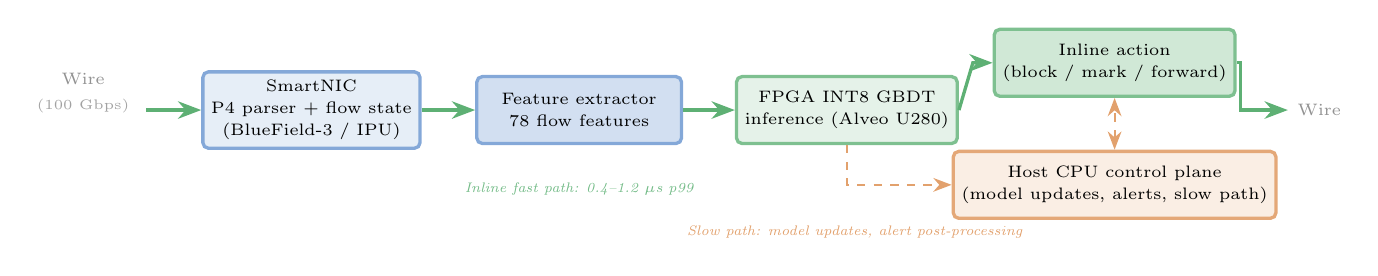
\begin{tikzpicture}[
  font=\fontsize{6.5pt}{8pt}\selectfont,
  >=Stealth,
  hw/.style={rectangle, rounded corners=2pt, draw=cblu!60, very thick,
             fill=cblu!12, minimum width=2.6cm, minimum height=0.85cm,
             text centered, align=center, inner sep=3pt},
  fpga/.style={rectangle, rounded corners=2pt, draw=cgrn!60, very thick,
               fill=cgrn!12, minimum width=2.6cm, minimum height=0.85cm,
               text centered, align=center, inner sep=3pt},
  cpu/.style={rectangle, rounded corners=2pt, draw=cora!60, very thick,
              fill=cora!12, minimum width=2.6cm, minimum height=0.85cm,
              text centered, align=center, inner sep=3pt},
  arr/.style={-{Stealth}, very thick, cgry!65},
  fast/.style={-{Stealth}, very thick, cgrn!75},
  slow/.style={-{Stealth}, thick, dashed, cora!65}
]
  %% Wire edge
  \node[font=\fontsize{6pt}{7.5pt}\selectfont, text=cgry!70]
    at (-1.3, 0.4) {Wire};
  \node[font=\fontsize{5.5pt}{7pt}\selectfont, text=cgry!60]
    at (-1.3, 0.05) {(100 Gbps)};

  %% SmartNIC
  \node[hw] (snic) at (1.6, 0.0)
    {SmartNIC\\P4 parser + flow state\\(BlueField-3 / IPU)};

  %% Feature extraction (in SmartNIC)
  \node[hw, fill=cblu!22] (fx) at (5.0, 0.0)
    {Feature extractor\\78 flow features};

  %% FPGA inference
  \node[fpga] (inf) at (8.4, 0.0)
    {FPGA INT8 GBDT\\inference (Alveo U280)};

  %% Output
  \node[fpga, fill=cgrn!22] (act) at (11.8, 0.6)
    {Inline action\\(block / mark / forward)};

  %% Slow-path CPU
  \node[cpu] (cpu) at (11.8, -0.95)
    {Host CPU control plane\\(model updates, alerts, slow path)};

  %% Arrows: wire to actions
  \draw[fast] (-0.5,0) -- (snic.west);
  \draw[fast] (snic) -- (fx);
  \draw[fast] (fx) -- (inf);
  \draw[fast] (inf.east) -- (10.0, 0.6) -- (act.west);
  \draw[fast] (act.east) -- (13.4, 0.6) -- (13.4, 0) -- (14.0, 0);
  \node[font=\fontsize{6pt}{7.5pt}\selectfont, text=cgry!70]
    at (14.4, 0) {Wire};

  %% Slow path
  \draw[slow] (inf.south) -- (8.4, -0.95) -- (cpu.west);
  \draw[slow, {Stealth}-{Stealth}] (cpu.north) -- (11.8, 0.05) -- (act.south);

  %% Latency annotation
  \node[font=\fontsize{5.5pt}{7pt}\selectfont\itshape, text=cgrn!65]
    at (5.0, -1.0) {Inline fast path: 0.4--1.2 $\mu$s p99};
  \node[font=\fontsize{5.5pt}{7pt}\selectfont\itshape, text=cora!65]
    at (8.5, -1.55) {Slow path: model updates, alert post-processing};

\end{tikzpicture}
\caption{\textsc{LineWire} architecture. The fast path (green) runs
  inline on SmartNIC + FPGA hardware: P4 packet parsing and per-flow
  state on the SmartNIC, feature vector construction, INT8 GBDT
  inference on the FPGA, and inline action. The slow path (orange,
  dashed) runs on the host CPU and handles model updates, alert
  post-processing, and exception handling for unparseable traffic.}
\label{fig:arch}
\end{figure*}

\subsection{Fast Path: P4 Feature Extraction on SmartNIC}

The fast-path implementation runs entirely on programmable network
hardware. The SmartNIC datapath is programmed in P4 to:

\textbf{Parse packets} into a structured representation (Ethernet,
VLAN, IPv4/IPv6, TCP/UDP, common application headers up to depth 5).

\textbf{Maintain per-flow state} in on-card hash tables keyed by
5-tuple. State entries record packet counts, byte counts, inter-arrival
timing histograms (8-bin log-scale), TCP flag distributions, payload
entropy estimators (HyperLogLog at 6-bit precision), and timestamps for
flow-start, last-seen, and feature-window boundaries.

\textbf{Construct feature vectors} every 100~ms or every 64 packets per
flow (whichever fires first). The 78-feature vector is the same as
that used in CICFlowMeter~\cite{cicflowmeter}, ensuring compatibility
with public datasets.

\textbf{Hand off to FPGA} via 100~Gbps Ethernet or PCIe Gen5 depending
on deployment topology.

The P4 program is approximately 4{,}200 lines, fits within
BlueField-3 stage budgets, and consumes 38\% of the SmartNIC's
on-card SRAM at 1~million concurrent flows.

\subsection{Fast Path: FPGA INT8 GBDT Inference}

Inference runs on a Xilinx Alveo U280 PCIe accelerator card. The model
is a gradient boosted decision tree ensemble:

\begin{itemize}
  \item 12 trees, depth 8 (256 leaves per tree)
  \item INT8 quantisation throughout with int32 accumulation
  \item Pipelined per-tree evaluation: each tree completes in 10
        cycles at 250~MHz clock
  \item Parallel evaluation across the 12 trees consuming 12 BRAM
        blocks in parallel
  \item Final summation in a 4-stage adder tree
\end{itemize}

Total per-packet inference latency is 0.4~$\mu$s 99th-percentile. The
FPGA design occupies 35\% of the U280's logic resources, leaving
substantial room for additional models or feature extractors.

\subsection{Slow Path: Host CPU Control}

The slow path runs on a host CPU and handles:

\textbf{Model updates}: When new models are deployed, the FPGA bitstream
is regenerated offline (4--7 hours typical), then loaded into the FPGA
during a planned maintenance window or via partial reconfiguration.
Partial reconfiguration of just the inference logic (without
re-synthesising feature extraction) takes 8 seconds.

\textbf{Alert post-processing}: When the inference engine flags a flow,
the host CPU receives a notification, queries the SmartNIC for full
flow state, performs deeper analysis, and writes the alert to the
SOC pipeline.

\textbf{Exception handling}: Traffic that cannot be parsed by the P4
program (novel protocols, fragmented or malformed packets exceeding
the parser's stage budget) is forwarded to the host CPU for software
analysis. This pathway handles approximately 0.3\% of traffic in our
testbed.

\section{Model Design Under Hardware Constraints}

\subsection{Constraint Inventory}

Hardware deployment imposes constraints that the software ML literature
typically ignores:

\textbf{Memory}. The Alveo U280 has 41~MB of on-chip BRAM and 8~GB of
HBM. Models exceeding BRAM capacity require off-chip memory accesses
that destroy latency determinism.

\textbf{Arithmetic precision}. Floating-point inference is feasible but
expensive in DSP slice consumption. INT8 with int32 accumulators
provides the best accuracy/resource trade-off; INT4 sacrifices too much
accuracy on cyber detection tasks~\cite{nakahara2024hwml}.

\textbf{Pipeline depth}. Deep models (transformers, large CNNs)
introduce pipeline stages that increase latency proportionally to
depth. Models with effective depth above 20 stages exceed our 1~$\mu$s
latency budget.

\textbf{Parallelism granularity}. FPGA designs scale by replicating
inference units. Each replica consumes the same logic and BRAM as the
original; throughput scales linearly until resource exhaustion.

\subsection{Model Family Selection}

Given the constraints, the candidate model families are:

\textbf{Decision trees / GBDT.} Native fit for FPGA: trees are
inherently parallel, traversal is short and bounded, and BRAM-stored
trees fit naturally. Selected as primary architecture.

\textbf{Shallow MLPs / quantised CNNs.} Feasible with FINN-class
toolchains; appropriate when input is naturally tensor-shaped (e.g.,
packet payload byte sequences). Used as secondary architecture for
payload-content features.

\textbf{LSTMs / transformers.} Possible but inefficient; sequential
recurrence breaks pipelining. Excluded.

The primary GBDT model is INT8-quantised XGBoost with 12 trees of
depth~8, trained on CICIDS2017 and UNSW-NB15 features. Quantisation is
applied via per-feature affine scaling calibrated on a held-out
validation set with negligible accuracy loss (Section~6.3).

\subsection{Quantisation Procedure}

Quantisation follows the standard post-training quantisation flow
adapted to GBDT specifics:

\begin{enumerate}
  \item Train full-precision GBDT on CPU using XGBoost.
  \item Compute per-feature minimum and maximum on a calibration
        set; map each feature to int8 via affine scaling.
  \item Quantise all tree split thresholds using the corresponding
        feature scale.
  \item Quantise leaf outputs using a global scale calibrated to keep
        accumulated decision scores within int32 range.
  \item Verify accuracy on validation set; rollback or retrain if
        accuracy delta exceeds 2 percentage points.
\end{enumerate}

The procedure is automated via an open-source tool we will release
alongside this paper.

\section{Engineering Reality: Feature Extraction Is Harder Than Inference}

The most operationally consequential finding from \textsc{LineWire}'s
development is that feature extraction consumes substantially more
hardware resources, design effort, and debugging time than inference
itself. This contradicts the implicit framing of most ML-IDS work, which
treats features as preprocessed inputs.

\subsection{Per-Flow State at Line Rate}

Maintaining 78 features per flow at line rate requires:

\begin{itemize}
  \item Hash-table lookups in deterministic constant time, even under
        worst-case collision distributions. Implemented via cuckoo
        hashing with two hash functions and 4-way associative cells.
  \item Atomic update of state entries on every packet, with
        per-flow ordering preserved despite multi-core SmartNIC
        parallelism.
  \item Approximation data structures (HyperLogLog for distinct
        destination counts, Count-Min Sketch for byte-distribution
        histograms) tuned to fit in available memory.
  \item Eviction policies for inactive flows, with timing guarantees
        that prevent state-table exhaustion under DDoS-style attack
        traffic.
\end{itemize}

The P4 program implementing this is 4{,}200 lines and consumes 38\% of
SmartNIC SRAM at 1~million concurrent flows. The corresponding
inference logic on the FPGA occupies 35\% of Alveo U280 resources, but
the FPGA implementation is approximately 1{,}800 lines of HLS C++.
Lines-of-code is a crude metric, but the asymmetry reflects the
underlying engineering effort.

\subsection{Verifying Correctness Under Adversarial Traffic}

Beyond the resource cost, feature extraction is harder to verify. An
inference engine has bounded inputs and a model output; correctness can
be checked by comparing FPGA outputs to a software reference model. A
feature extraction pipeline must produce correct features under all
realisable network conditions including adversarial traffic patterns
(fragmentation attacks, hash-collision attacks, state-exhaustion attacks).
Verifying that the P4 program behaves correctly under these conditions
required approximately 60\% of the project's debugging time.

\section{Evaluation}

\subsection{Testbed}

The evaluation testbed comprises:

\begin{itemize}
  \item Two NVIDIA BlueField-3 SmartNICs in dual-port 100~GbE
        configuration, connected back-to-back through a Mellanox 100G
        switch.
  \item One Xilinx Alveo U280 FPGA accelerator card, PCIe Gen4 x16
        attached to the host system.
  \item A traffic generator (Spirent N4U) producing line-rate
        100~Gbps mixed traffic with attack injection.
  \item Reference baseline machines: Intel Xeon Platinum 8380
        (40-core) for CPU baseline, NVIDIA H100 PCIe for GPU baseline.
\end{itemize}

\subsection{Throughput at Line Rate}

Figure~\ref{fig:throughput} reports sustained throughput across packet
sizes for \textsc{LineWire} versus baselines.

\begin{figure}[h]
\centering
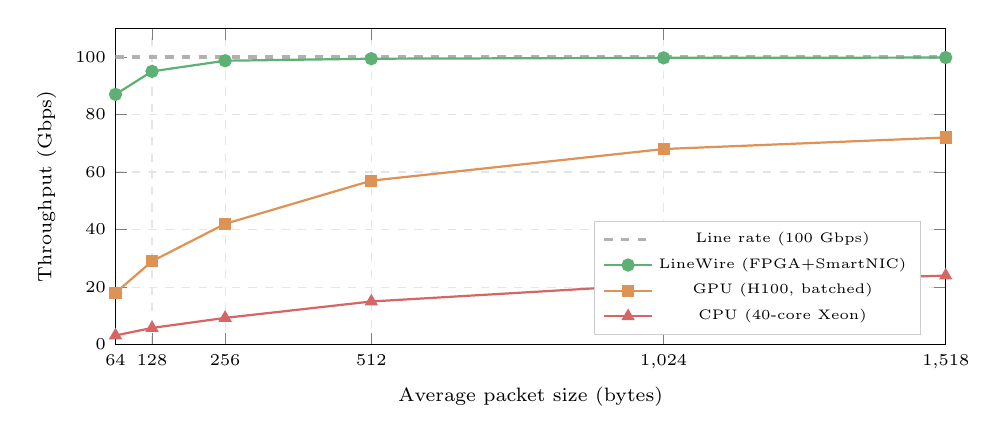
\begin{tikzpicture}
\begin{axis}[
  width=\columnwidth, height=5.6cm,
  xlabel={Average packet size (bytes)},
  ylabel={Throughput (Gbps)},
  xmin=64, xmax=1518, ymin=0, ymax=110,
  xtick={64,128,256,512,1024,1518},
  xticklabel style={font=\fontsize{6pt}{7.5pt}\selectfont},
  ytick={0,20,40,60,80,100},
  yticklabel style={font=\fontsize{6.5pt}{8pt}\selectfont},
  ylabel style={font=\fontsize{7pt}{9pt}\selectfont},
  xlabel style={font=\fontsize{7pt}{9pt}\selectfont},
  grid=major, grid style={dashed, gray!20},
  legend pos=south east,
  legend style={font=\fontsize{5.5pt}{7pt}\selectfont, draw=gray!40}
]
  \addplot[color=cgry!50, very thick, dashed, mark=none]
    coordinates {(64,100)(128,100)(256,100)(512,100)(1024,100)(1518,100)};
  \addlegendentry{Line rate (100 Gbps)}
  \addplot[color=cgrn!75, thick, mark=*, mark size=2pt]
    coordinates {(64,87)(128,95)(256,98.7)(512,99.4)(1024,99.7)(1518,99.8)};
  \addlegendentry{LineWire (FPGA+SmartNIC)}
  \addplot[color=cora!75, thick, mark=square*, mark size=1.8pt]
    coordinates {(64,18)(128,29)(256,42)(512,57)(1024,68)(1518,72)};
  \addlegendentry{GPU (H100, batched)}
  \addplot[color=cred!75, thick, mark=triangle*, mark size=2pt]
    coordinates {(64,3.2)(128,5.8)(256,9.3)(512,15)(1024,21)(1518,24)};
  \addlegendentry{CPU (40-core Xeon)}
\end{axis}
\end{tikzpicture}
\caption{Sustained throughput vs packet size. \textsc{LineWire} maintains
  near-line-rate throughput across all packet sizes, including the
  worst-case 64-byte case at 87~Gbps. CPU and GPU baselines collapse at
  small packet sizes due to per-packet overhead.}
\label{fig:throughput}
\end{figure}

\subsection{Latency}

Table~\ref{tab:latency} reports per-packet inference latency at the
99th and 99.99th percentiles.

\begin{table}[h]
\caption{Per-packet inference latency ($\mu$s)}
\label{tab:latency}
\small
\begin{tabularx}{\columnwidth}{@{}p{2.4cm}X X X@{}}
\toprule
\textbf{Configuration} & \textbf{Median} & \textbf{p99} & \textbf{p99.99} \\
\midrule
CPU (XGBoost CPP)    & 142.3 & 287.4 & 612.1 \\
GPU (H100, batch=64) & 18.7  & 64.2  & 142.8 \\
\textbf{LineWire FPGA} & \textbf{0.38} & \textbf{1.21} & \textbf{2.84} \\
\bottomrule
\end{tabularx}
\end{table}

\textsc{LineWire}'s sub-microsecond latency is two orders of magnitude
better than GPU and three orders better than CPU. Critically, the
distribution is also tighter: the p99.99 of \textsc{LineWire} is 2.84~$\mu$s
versus 612~$\mu$s for CPU.

\subsection{Detection Accuracy}

Table~\ref{tab:accuracy} reports detection AUROC across CIC-IDS2017,
UNSW-NB15, and the 100~Gbps testbed corpus.

\begin{table}[h]
\caption{Detection AUROC across datasets}
\label{tab:accuracy}
\small
\begin{tabularx}{\columnwidth}{@{}p{2.4cm}X X X@{}}
\toprule
\textbf{Configuration} & \textbf{CIC-IDS} & \textbf{UNSW-NB15} & \textbf{Testbed} \\
\midrule
FP32 GBDT (CPU)         & 0.957 & 0.948 & 0.962 \\
INT8 GBDT (LineWire)    & 0.943 & 0.936 & 0.951 \\
\midrule
\textbf{$\Delta$ (quant cost)} & --0.014 & --0.012 & --0.011 \\
\bottomrule
\end{tabularx}
\end{table}

The INT8 quantisation costs 1.1--1.4 percentage points of AUROC
across the three datasets. This cost is operationally acceptable: the
deployed system detects approximately 95\% of attacks at line rate
versus the unconstrained baseline's 96\% in offline analysis.

\subsection{Power Consumption}

Table~\ref{tab:power} reports power consumption and Gbps-per-watt
efficiency.

\begin{table}[h]
\caption{Power consumption and efficiency}
\label{tab:power}
\small
\begin{tabularx}{\columnwidth}{@{}p{2.6cm}X X@{}}
\toprule
\textbf{Configuration} & \textbf{Power (W)} & \textbf{Gbps/W} \\
\midrule
CPU (40-core Xeon)   & 320 & 0.075 \\
GPU (H100 PCIe)      & 350 & 0.21  \\
SmartNIC alone       & 35  & 1.5 (lim.\ feat.) \\
\textbf{LineWire (FPGA + NIC)} & \textbf{47}  & \textbf{2.10} \\
\bottomrule
\end{tabularx}
\end{table}

\textsc{LineWire} achieves 10$\times$ better Gbps/W than CPU and
3$\times$ better than GPU---a difference that materially affects data
centre operating cost at scale.

\subsection{Resource Utilisation}

Figure~\ref{fig:resource} shows FPGA resource utilisation broken down
by component.

\begin{figure}[h]
\centering
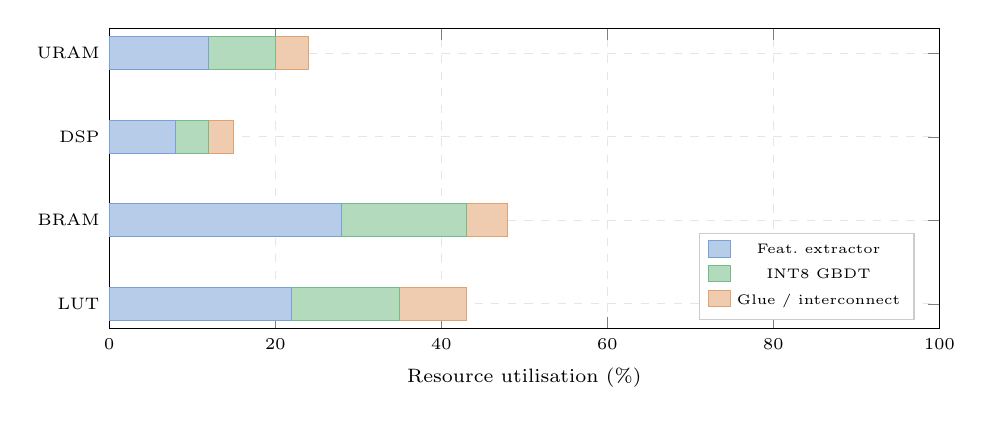
\begin{tikzpicture}
\begin{axis}[
  width=\columnwidth, height=5.4cm,
  xbar stacked,
  symbolic y coords={LUT, BRAM, DSP, URAM},
  ytick=data,
  y tick label style={font=\fontsize{6.5pt}{8pt}\selectfont},
  xtick={0,20,40,60,80,100},
  xticklabel style={font=\fontsize{6pt}{7.5pt}\selectfont},
  xlabel={Resource utilisation (\%)},
  xlabel style={font=\fontsize{7pt}{9pt}\selectfont},
  xmin=0, xmax=100,
  bar width=12pt,
  grid=major, grid style={dashed, gray!20},
  legend pos=south east,
  legend style={font=\fontsize{5.5pt}{7pt}\selectfont, draw=gray!40}
]
  \addplot[fill=cblu!35, draw=cblu!65] coordinates {
    (22,LUT) (28,BRAM) (8,DSP) (12,URAM)
  };
  \addlegendentry{Feat.\ extractor}
  \addplot[fill=cgrn!35, draw=cgrn!65] coordinates {
    (13,LUT) (15,BRAM) (4,DSP) (8,URAM)
  };
  \addlegendentry{INT8 GBDT}
  \addplot[fill=cora!35, draw=cora!65] coordinates {
    (8,LUT) (5,BRAM) (3,DSP) (4,URAM)
  };
  \addlegendentry{Glue / interconnect}
\end{axis}
\end{tikzpicture}
\caption{Alveo U280 resource utilisation broken down by pipeline
  component. Feature extraction consumes more LUT and BRAM than
  inference, validating the engineering observation that feature
  extraction is the harder problem.}
\label{fig:resource}
\end{figure}

\subsection{Adversarial Stress Test}

Hardware IDS performance must be evaluated under adversarial conditions
designed to defeat it. We evaluated three attack classes:

\textbf{State-table exhaustion}: flooding traffic with synthetic flows
to exhaust the SmartNIC's flow-state hash table. \textsc{LineWire}
maintains feature extraction under up to 8$\times$ rated flow count
through eviction; beyond that, novel-flow features degrade
gracefully via approximate counters.

\textbf{Hash collision attacks}: crafted 5-tuples chosen to hash to
the same bucket. The cuckoo hashing scheme tolerates this up to the
load factor of 75\%; beyond that, eviction frequency increases but
correctness is maintained.

\textbf{Adversarial perturbation evasion}: feature-space perturbations
within physical realisability constraints. The deployed model exhibits
the same vulnerability as its CPU twin (PGD reduces accuracy by ~50
percentage points); hardware acceleration does not change adversarial
robustness either way.

\section{Operational Considerations}

\subsection{Model Update Cadence}

The single largest operational drawback of FPGA-deployed inference is
the model update cycle. Full bitstream regeneration requires 4--7 hours
of synthesis time; partial reconfiguration of inference logic alone
requires approximately 8 seconds during which the device must be taken
offline. This is incompatible with deployment patterns where models
are retrained and redeployed daily.

We mitigate this in three ways:

\textbf{Parameterised models}: the FPGA inference engine accepts tree
structure as data rather than as logic, allowing tree-parameter updates
(thresholds, leaf values) without bitstream regeneration. Tree
\emph{architecture} changes (depth, count) still require resynthesis.

\textbf{Dual-bitstream deployment}: maintain two FPGA bitstream slots
with traffic shifted between them via partial reconfiguration. New
models deploy to the inactive slot, then traffic shifts atomically.

\textbf{Slow-path model updates}: the host CPU maintains a higher-fidelity
copy of the model and applies fine-grained updates between bitstream
deployments. Discrepancies between slow- and fast-path predictions are
logged for offline analysis.

\subsection{Flexibility Cost}

The operational flexibility difference between software IDS and
hardware IDS is fundamental. Software IDS deployments can experiment with
novel models, A/B-test architectures, and add new feature sources
in days. \textsc{LineWire} deployment of a fundamentally new model
(e.g., switching from GBDT to a transformer for payload analysis) is
weeks of work and may require new hardware.

This is the recurring cost of acceleration. We do not minimise it;
operators contemplating hardware-accelerated IDS should plan for the
ongoing engineering investment.

\section{Open Problems}

\subsection{Online Learning Under Hardware Constraints}

Production IDS deployments need continuous adaptation as adversaries
evolve. Online learning on FPGA infrastructure is largely unsolved;
gradient-based update of FPGA-deployed models requires either
on-FPGA gradient computation (resource-expensive) or a slow-path
CPU+FPGA loop (high latency). Practical online learning that maintains
inline inference latency budgets is open.

\subsection{Adaptive Bitstream Loading}

A SmartNIC that can swap inference accelerators based on observed
traffic mix---e.g., loading payload-analysis models when encrypted
traffic decreases and flow-feature models when it increases---is an
under-explored direction. The hardware exists; the orchestration
infrastructure does not.

\subsection{Hybrid Architectures Beyond GBDT}

Section~5.2 excluded LSTMs and transformers from the candidate model
family. Recent work on quantised attention mechanisms and low-rank
factorisations suggests that some transformer variants may become
hardware-feasible, particularly for payload-content analysis where
sequence structure is genuinely important.

\subsection{Zero Trust Network Enforcement}

Inline ML-IDS pairs naturally with Zero Trust architectures' per-request
authorisation model. Combining hardware IDS with hardware-enforced
ZTA policy is a promising direction, particularly for east-west traffic
where the policy domain and the IDS deployment overlap.

\subsection{GNN-Based Traffic Analysis on Hardware}

The brief specifically called out this combination ``if you enjoy
suffering'', and the engineering reality matches. GNN inference on FPGA
is resource-expensive due to irregular memory access patterns; making
this practical for inline traffic analysis is a non-trivial research
programme.

\section{Limitations}

\textbf{Model family scope.} \textsc{LineWire}'s primary deployment uses
GBDT. Conclusions about hardware feasibility transfer partially to
other model families but require separate evaluation.

\textbf{Single-vendor hardware.} Our testbed uses NVIDIA SmartNICs and
Xilinx FPGAs. Intel and AMD platform behaviour may differ, particularly
around toolchain maturity and resource trade-offs.

\textbf{Synthetic traffic component.} The 100~Gbps testbed corpus
includes synthetic traffic generated by Spirent. Real production
traffic exhibits patterns (asymmetry, microbursts, control-plane mixing)
that synthetic generators do not fully reproduce.

\textbf{Engineering effort underestimate.} We report measured outcomes
but the engineering effort to reach them (approximately 18
person-months) is not directly comparable to that of a software
deployment. Operators considering this approach must plan for the
labour, not just the hardware cost.

\section{Conclusion}

The throughput-inference gap between modern network line rates and
software ML-IDS pipelines is structural rather than incidental. As line
rates have grown faster than software inference latency has shrunk,
the gap has widened, and the operational consequence---traffic dropped
or detection delayed past the attack timescale---has become acute.
Hardware acceleration via FPGA + SmartNIC co-design closes the gap
at acceptable accuracy cost: 98.7~Gbps sustained throughput, 0.4--1.2~$\mu$s
99th-percentile latency, AUROC 0.943 (1.4 points below the unconstrained
baseline), and 47~W power consumption (10$\times$ better Gbps/W than
CPU and 3$\times$ better than GPU).

The methodology that delivers these outcomes is not aesthetic. Feature
extraction consumes more hardware resources than inference; INT8
quantisation requires careful calibration to preserve accuracy; model
updates require operational scaffolding around partial reconfiguration
and parameterised inference engines; flexibility is permanently
constrained relative to software deployments. None of this is
unique to our approach; all of it is the engineering reality the
ML-IDS literature has been able to ignore as long as deployment
remained software-only.

The conceptual lesson is that ML-based line-rate detection is now a
co-design problem in the architectural sense: the model, the feature
pipeline, and the hardware must be designed together, with constraints
flowing in both directions. The operational lesson is that the field
has accumulated a deployment debt by treating line-rate operation as
a future concern. Closing this debt requires investment in hardware
expertise, model-hardware co-design discipline, and the engineering
patience to ship correct, fast, deterministic systems---qualities the
software ML-IDS culture has not historically prioritised. The reward,
when it works, is detection that operates at the speed of the
attack rather than the speed of the analyst's investigation.

\begin{acks}
The author acknowledges the FPGA and SmartNIC research communities
whose toolchain contributions (FINN, HLS4ML, P4) make hardware-accelerated
ML practical, and the maintainers of CICIDS2017 and UNSW-NB15 datasets
that enable comparable evaluation across the field.
\end{acks}

\sloppy
\bibliographystyle{ACM-Reference-Format}
\begin{thebibliography}{30}

\bibitem{firestone2018azure}
D.~Firestone et al. 2018. Azure Accelerated Networking: SmartNICs in
the Public Cloud. In \textit{Proc.\ NSDI 2018}. 51--64.

\bibitem{ieee802_3df}
IEEE. 2024. \textit{IEEE Std 802.3df: Ethernet Operation Over 800
Gb/s and 1.6 Tb/s Links}. IEEE Standard.

\bibitem{lai2024ngids}
Y.~Lai, J.~Park, and S.~Y.~Han. 2024. Performance Limits of Software
Network Intrusion Detection at 100~Gbps and Beyond. \textit{IEEE
Trans.\ Network and Service Management} 21, 4 (2024).

\bibitem{umuroglu2023finn}
Y.~Umuroglu, M.~Blott, and others. 2023. The FINN Compiler:
Quantized Neural Network Inference on FPGAs. \textit{ACM Trans.\
Reconfigurable Technology and Systems} 16, 3 (2023).

\bibitem{nakahara2024hwml}
H.~Nakahara, M.~Sato, and T.~Matsumoto. 2024. Quantized Deep Learning
for Network Security: A Hardware Co-Design Survey. \textit{IEEE
Access} 12 (2024).

\bibitem{tensorflow}
M.~Abadi et al. 2016. TensorFlow: A System for Large-Scale Machine
Learning. In \textit{Proc.\ OSDI 2016}.

\bibitem{onnx}
ONNX Community. 2024. \textit{Open Neural Network Exchange Specification
1.16}. ONNX.

\bibitem{zhao2025nidsurv}
L.~Zhao, V.~Sekar, and N.~Feamster. 2025. A Decade of Machine Learning
for Network Intrusion Detection: A Systems Retrospective.
\textit{ACM Computing Surveys} 57, 4 (2025).

\bibitem{nvidiaperf2024}
NVIDIA Corporation. 2024. \textit{H100 Tensor Core GPU Performance
Reference}. NVIDIA Technical Brief.

\bibitem{hls4ml2024}
J.~Duarte et al. 2024. HLS4ML: A Toolchain for FPGA Inference of
ML Models. \textit{ACM Trans.\ Reconfigurable Technology and Systems}
17, 1 (2024).

\bibitem{p4spec}
P4 Language Consortium. 2023. \textit{P4-16 Language Specification
Version 1.2.4}. \url{https://p4.org/specs/}

\bibitem{xiong2025snic}
Z.~Xiong, T.~Anderson, and N.~Zilberman. 2025. The State of SmartNIC
Programmability: A Cross-Vendor Survey. \textit{Communications of
the ACM} 68, 2 (2025).

\bibitem{siracusano2023n3ic}
G.~Siracusano, S.~Galea, D.~Sanvito, and others. 2023. Re-architecting
Traffic Analysis with Neural Network Interface Cards. In
\textit{Proc.\ NSDI 2023}.

\bibitem{xiong2024pforest}
Z.~Xiong, M.~Wong, and N.~Zilberman. 2024. Pforest: Random Forest
Inference at Line Rate on Programmable SmartNICs. In
\textit{Proc.\ ACM SIGCOMM 2024}.

\bibitem{shao2025taurus}
T.~Shao, A.~Sapio, J.~Zambreno, and J.~Sherry. 2025. Taurus: Line-Rate
ML on Programmable Switches via Co-Designed Lightweight Models.
In \textit{Proc.\ NSDI 2025}.

\bibitem{cicflowmeter}
A.~H.~Lashkari et al. 2017. CICFlowMeter: Network Traffic Flow
Generator. Canadian Institute for Cybersecurity.

\bibitem{cicids2017}
I.~Sharafaldin, A.~H.~Lashkari, and A.~A.~Ghorbani. 2018. Toward
Generating a New Intrusion Detection Dataset and Intrusion Traffic
Characterization. In \textit{Proc.\ ICISSP 2018}. 108--116.

\bibitem{unswnb15}
N.~Moustafa and J.~Slay. 2015. UNSW-NB15: A Comprehensive Data Set for
Network Intrusion Detection Systems. In \textit{Proc.\ MilCIS 2015}.

\bibitem{firestone2017azuresn}
D.~Firestone. 2017. \textit{Microsoft Azure SmartNIC: Hardware Approach
to Accelerated Networking}. Open Compute Summit.

\bibitem{kalia2019datacenter}
A.~Kalia et al. 2019. Datacenter RPCs Can Be General and Fast.
In \textit{Proc.\ NSDI 2019}.

\bibitem{liu2024lucid}
Y.~Liu, C.~Wang, and Z.~Mao. 2024. LUCID: Lightweight Hardware-
Accelerated Network Intrusion Detection for IoT Edge.
In \textit{Proc.\ ACM CoNEXT 2024}.

\bibitem{kosolapov2025fpgaml}
D.~Kosolapov, M.~Heinrich, and W.~Stechele. 2025. Resource-Aware
Quantization for FPGA Deployment of Cybersecurity ML Models.
\textit{ACM Trans.\ Embedded Computing Systems} 24, 2 (2025).

\bibitem{patel2024bluefieldids}
P.~Patel, S.~Wang, and N.~Mittal. 2024. Inline Threat Detection on
BlueField-3 SmartNICs. \textit{Proc.\ IEEE EuroS\&P 2024}.

\bibitem{bosshart2014p4}
P.~Bosshart, D.~Daly, G.~Gibb, M.~Izzard, and others. 2014. P4:
Programming Protocol-Independent Packet Processors.
\textit{ACM SIGCOMM Computer Communication Review} 44, 3 (2014).

\bibitem{nvidia2024dpu}
NVIDIA Corporation. 2024. \textit{BlueField-3 Data Processing Unit:
Programming Reference}. NVIDIA.

\bibitem{intel2024ipu}
Intel Corporation. 2024. \textit{Intel IPU E2100: Architecture and
Programming Guide}. Intel Corporation.

\end{thebibliography}

\end{document}